%package list
\documentclass{article}
\usepackage[top=3cm, bottom=3cm, outer=3cm, inner=3cm]{geometry}
\usepackage{multicol}
\usepackage{graphicx}
\usepackage{url}
%\usepackage{cite}
\usepackage{hyperref}
\usepackage{array}
%\usepackage{multicol}
\newcolumntype{x}[1]{>{\centering\arraybackslash\hspace{0pt}}p{#1}}
\usepackage{natbib}
\usepackage{pdfpages}
\usepackage{multirow}
\usepackage[normalem]{ulem}
\useunder{\uline}{\ul}{}
\usepackage{svg}
\usepackage{xcolor}
\usepackage{listings}
\lstdefinestyle{ascii-tree}{
    literate={├}{|}1 {─}{--}1 {└}{+}1 
  }
\lstset{basicstyle=\ttfamily,
  showstringspaces=false,
  commentstyle=\color{red},
  keywordstyle=\color{blue}
}
%\usepackage{booktabs}
\usepackage{caption}
\usepackage{subcaption}
\usepackage{float}
\usepackage{array}

\newcolumntype{M}[1]{>{\centering\arraybackslash}m{#1}}
\newcolumntype{N}{@{}m{0pt}@{}}


%%%%%%%%%%%%%%%%%%%%%%%%%%%%%%%%%%%%%%%%%%%%%%%%%%%%%%%%%%%%%%%%%%%%%%%%%%%%
%%%%%%%%%%%%%%%%%%%%%%%%%%%%%%%%%%%%%%%%%%%%%%%%%%%%%%%%%%%%%%%%%%%%%%%%%%%%
\newcommand{\itemEmail}{vmamanian@unsa.edu.pe}
\newcommand{\itemStudent}{Victor Mamani Anahua}
\newcommand{\itemCourse}{Fundamentos de la Programación II}
\newcommand{\itemCourseCode}{20230489}
\newcommand{\itemSemester}{II}
\newcommand{\itemUniversity}{Universidad Nacional de San Agustín de Arequipa}
\newcommand{\itemFaculty}{Facultad de Ingeniería de Producción y Servicios}
\newcommand{\itemDepartment}{Departamento Académico de Ingeniería de Sistemas e Informática}
\newcommand{\itemSchool}{Escuela Profesional de Ingeniería de Sistemas}
\newcommand{\itemAcademic}{2023 - B}
\newcommand{\itemInput}{Del 17 Octubre 2023}
\newcommand{\itemOutput}{Al 24 Octubre 2023}
\newcommand{\itemPracticeNumber}{08}
\newcommand{\itemTheme}{Laboratorio 08}
%%%%%%%%%%%%%%%%%%%%%%%%%%%%%%%%%%%%%%%%%%%%%%%%%%%%%%%%%%%%%%%%%%%%%%%%%%%%
%%%%%%%%%%%%%%%%%%%%%%%%%%%%%%%%%%%%%%%%%%%%%%%%%%%%%%%%%%%%%%%%%%%%%%%%%%%%

\usepackage[english,spanish]{babel}
\usepackage[utf8]{inputenc}
\AtBeginDocument{\selectlanguage{spanish}}
\renewcommand{\figurename}{Figura}
\renewcommand{\refname}{Referencias}
\renewcommand{\tablename}{Tabla} %esto no funciona cuando se usa babel
\AtBeginDocument{%
	\renewcommand\tablename{Tabla}
}

\usepackage{fancyhdr}
\pagestyle{fancy}
\fancyhf{}
\setlength{\headheight}{30pt}
\renewcommand{\headrulewidth}{1pt}
\renewcommand{\footrulewidth}{1pt}
\fancyhead[L]{\raisebox{-0.2\height}{
\includegraphics[width=3cm]{img/logo_episunsa.png}}}
\fancyhead[C]{\fontsize{7}{7}\selectfont	\itemUniversity \\ \itemFaculty \\ \itemDepartment \\ \itemSchool \\ \textbf{\itemCourse}}
\fancyhead[R]{\raisebox{-0.2\height}{
\includegraphics[width=1.2cm]{img/logo_abet}}}
\fancyfoot[L]{Estudiante Victor Mamani A.}
\fancyfoot[C]{\itemCourse}
\fancyfoot[R]{Página \thepage}

% para el codigo fuente
\usepackage{listings}
\usepackage{color, colortbl}
\definecolor{dkgreen}{rgb}{0,0.6,0}
\definecolor{gray}{rgb}{0.5,0.5,0.5}
\definecolor{mauve}{rgb}{0.58,0,0.82}
\definecolor{codebackground}{rgb}{0.95, 0.95, 0.92}
\definecolor{tablebackground}{rgb}{0.8, 0, 0}

\lstdefinestyle{java}{frame=tb,
	language=Java,
	showstringspaces=false,
	columns=flexible,
	basicstyle={\footnotesize\ttfamily\color[RGB]{255,255,255}},
	numberstyle=\color{mygray},
	numbers=left, 
	keywordstyle=\color{myblue},
	morekeywords={String, System},
	commentstyle=\color{mygray},
	stringstyle=\color{mygreen},
	breaklines=true,
	breakatwhitespace=true,
	tabsize=2,
	backgroundcolor= \color{codebackgroundCode},
	showspaces=false,
	showtabs=false,
	showlines=false,
}

\lstset{frame=tb,
	language=bash,
	aboveskip=3mm,
	belowskip=3mm,
	showstringspaces=false,
	columns=flexible,
	basicstyle={\small\ttfamily},
	numbers=none,
	numberstyle=\tiny\color{gray},
	keywordstyle=\color{blue},
	commentstyle=\color{dkgreen},
	stringstyle=\color{mauve},
	breaklines=true,
	breakatwhitespace=true,
	tabsize=3,
	backgroundcolor= \color{codebackground},
}

\begin{document}
	
	\vspace*{10px}
	
	\begin{center}	
		\fontsize{17}{17} \textbf{ Informe de Laboratorio \itemPracticeNumber}
	\end{center}
	\centerline{\textbf{\Large Tema: \itemTheme}}
	%\vspace*{0.5cm}	

	\begin{flushright}
		\begin{tabular}{|M{2.5cm}|N|}
			\hline 
			\rowcolor{tablebackground}
			\color{white} \textbf{Nota}  \\
			\hline 
			     \\[30pt]
			\hline 			
		\end{tabular}
	\end{flushright}	

	\begin{table}[H]
		\begin{tabular}{|x{4.7cm}|x{4.8cm}|x{4.8cm}|}
			\hline 
			\rowcolor{tablebackground}
			\color{white} \textbf{Estudiante} & \color{white}\textbf{Escuela}  & \color{white}\textbf{Asignatura}   \\
			\hline 
			{\itemStudent \par \itemEmail} & \itemSchool & {\itemCourse \par Semestre: \itemSemester \par Código: \itemCourseCode}     \\
			\hline 			
		\end{tabular}
	\end{table}		
	
	\begin{table}[H]
		\begin{tabular}{|x{4.7cm}|x{4.8cm}|x{4.8cm}|}
			\hline 
			\rowcolor{tablebackground}
			\color{white}\textbf{Laboratorio} & \color{white}\textbf{Tema}  & \color{white}\textbf{Duración}   \\
			\hline 
			\itemPracticeNumber & \itemTheme & 04 horas   \\
			\hline 
		\end{tabular}
	\end{table}
	
	\begin{table}[H]
		\begin{tabular}{|x{4.7cm}|x{4.8cm}|x{4.8cm}|}
			\hline 
			\rowcolor{tablebackground}
			\color{white}\textbf{Semestre académico} & \color{white}\textbf{Fecha de inicio}  & \color{white}\textbf{Fecha de entrega}   \\
			\hline 
			\itemAcademic & \itemInput &  \itemOutput  \\
			\hline 
		\end{tabular}
	\end{table}
	
	\section{Tarea}
	\begin{itemize}		
        \item Cree un Proyecto llamado Laboratorio8
		\item Usted deberá crear las dos clases Soldado.java y VideoJuego5.java. Puede reutilizar lo desarrollado en Laboratorios anteriores.
		\item Del Soldado nos importa el nombre, puntos de vida, fila y columna (posición en el tablero).
		\item El juego se desarrollará en el mismo tablero de los laboratorios anteriores. Para el tablero utilizar la estructura de datos más adecuada.
		\item Tendrá 2 Ejércitos (usar HashMaps). Inicializar el tablero con n soldados aleatorios entre 1 y 10 para cada Ejército. Cada soldado tendrá un nombre autogenerado: Soldado0X1, Soldado1X1, etc., un valor de puntos de vida autogenerado aleatoriamente [1..5], la fila y columna también autogenerados aleatoriamente (no puede haber 2 soldados en el mismo cuadrado). 
		\item Además de los datos del Soldado con mayor vida de cada ejército, el promedio de puntos de vida de todos los soldados creados por ejército, los datos de todos los soldados porejército en el orden que fueron creados y un ranking de poder de todos los soldados creados por ejército (del que tiene más nivel de vida al que tiene menos) usando 2 diferentes algoritmos de ordenamiento (indicar conclusiones respecto a este ordenamiento de HashMaps).
		\item Finalmente, que muestre qué ejército ganará la batalla (indicar la métrica usada para decidir al ganador de la batalla).
	\end{itemize}

	\section{Equipos, materiales y temas utilizados}
	\begin{itemize}
		\item Sistema Operativo Ubuntu GNU Linux 23 lunar 64 bits Kernell 6.2.v
		\item Visual Studio Code.
		\item VIM 9.0.
		\item OpenJDK 64-Bits 19.0.7.
		\item Git 2.39.2.
		\item Cuenta en GitHub con el correo institucional.
		\item Programación Orientada a Objetos.
		\item Actividades del Laboratorio 08.	
	\end{itemize}
	
	\section{URL de Repositorio Github}
	\begin{itemize}
		\item URL del Repositorio GitHub para clonar o recuperar.
		\item \url{https://github.com/VictorMA18/fp2-23b.git}
		\item URL para el laboratorio 08 en el Repositorio GitHub.
		\item \url{https://github.com/VictorMA18/fp2-23b/tree/main/Fase02/Lab08}
	\end{itemize}
	
	\section{Actividades del Laboratorio 08}
	
	\subsection{Ejercicio Soldado}
	\begin{itemize}	
		\item En el primer commit bueno reutilizamos el archivo que seria nuestra clase Soldado el cual la utilizaremos para poder avanzar con el siguiente ejercicio que seria VideoJuego5.
		\item El codigo y el commit seria el siguiente:
	\end{itemize}	
	\begin{lstlisting}[language=bash,caption={Commit}][H]
		$ git commit -m "Publicando la clase Soldado para su posterior uso en el siguiente ejercicio que es con Hashmaps"
	\end{lstlisting}	
	\begin{lstlisting}[language=java,caption={Las lineas de codigos del metodo creado:}][H]
		// Laboratorio Nro 8  - Ejercicio Soldado
		// Autor: Mamani Anahua Victor Narciso
		// Colaboro:
		// Tiempo:
		public class Soldado { //CREAMOS LA CLASE SOLDODADO PARA PODER USAR UN ARREGLO BIDIMENSIONAL DONDE NECESITAMOS LA VIDA , EL NOMBRE DEL SOLDADO Y TAMBIEN SU POSICION COMO LA FILA Y LA COLUMNA   

			private String name;
			private int heatlh; 
			private int row;
			private String column;

			//Constructor
			public Soldado(String name, int health, int row, String column){
			this.name = name;
			this.health = health;
			this.row = row;
			this.column = column;
			}

			// Metodos mutadores
			public void setName(String n){
				name = n;
			}
			public void setHealth(int p){
				heatlh = p;
			}
			public void setRow(int b){
				row = b;
			}
			public void setColumn(String c){
				column = c; 
			}

			// Metodos accesores
			public String getName(){
				return name;
			}
			public int getHealth(){
				return heatlh;

			}
			public int getRow(){
				return row;
			}
			public String getColumn(){
				return column;
			}

			// Completar con otros metodos necesarios
			public String toString(){ //CREAMOS ESTE METODO PARA IMPRIMIR LOS DATOS DEl OBJETO
				String join = "\nNombre: " + getName() + "\nVida: " + getHealth() + "\nFila: " + getRow() + "\nColumna: " + getColumn(); //Agregamos un espaciador para poder separar
				return join;
			}
		}
	\end{lstlisting}
	\subsection{Ejercicio VideoJuego5}
	\begin{itemize}	
		\item En el segundo commit creamos el metodo mapHashFillRegister() el cual usamos el uso de HashMaps y tambien de ArrayList para poder añadirlos al hashmaps ya que en este hariamos la comprobacion de que cada Soldado gracias a una iteracion el cual este comprueba que estos si son nulos se añadiria al soldado en la cuadrilla correspondiente y si no no lo añadiria y retrocederia una iteracion ya que se contaria por lo que nos lleva a que en este no se repita en misma cuadrilla despues de esto imprimiriamos los datos del soldado en el orden que fueron creados
		\item El codigo , el commit y la ejecucion seria el siguiente:
	\end{itemize}	
	\begin{lstlisting}[language=bash,caption={Commit}][H]
		$ git commit -m "Creando el metodo mapHashFillRegister() el cual usamos el uso de HashMaps y tambien de ArrayList para poder anadirlos al hashmaps ya que en este hariamos la comprobacion de que cada Soldado en este no se repita en misma cuadrilla despues de esto imprimiriamos los datos del soldado en el orden que fueron creados"
	\end{lstlisting}	
	\begin{lstlisting}[language=java,caption={Las lineas de codigos del metodo creado:}][H]
		public static void viewBoard(HashMap<String, Soldado> army1, HashMap<String, Soldado> army2){ //EN ESTE METODO DEMOSTRAREMOS LA TABLA REUTILIZAREMOS CODIGOS DE ANTERIORES LABORATORIOS PARA PODER HACER LA BASE DE ESTE TABLERO
			System.out.println("\nMostrando tabla de posicion ... --");
			System.out.println("Leyenda: Ejercito1 --> X | Ejercito2 --> Y"); //RECONOCIMIENTO PARA LOS EJERCITOS Y POSICION DE SUS SOLDADOS
			System.out.println("\n \t   A\t   B\t   C\t   D\t   E\t   F\t   G\t   H\t   I\t   J"); // RECONOCIMIENTO PARA CADA UBICACION DE CADA SOLDADO EN EL TABLERO POR PARTE DE LAS COLUMNAS
			System.out.println("\t_________________________________________________________________________________");
			for(int i = 0; i < 10; i++ ){
				System.out.print((i + 1) + "\t"); // RECONOCIMIENTO PARA CADA UBICACION DE CADA SOLDADO EN EL TABLERO POR PARTE DE LAS FILAS
					for(int j = 0; j < 10; j++){
							if(army1.get("Soldado" + i + "X" + j) != null){
								System.out.print("|   " + "X" + "   "); //VERIFICANDOLA POSICIONES DE CADA SOLDADO DE CADA EJERCITO CON SU RESPECTIVO INDICADOR PARA PODER UBICARLOS
							}else if(army2.get("Soldado" + i + "X" + j) != null){
								System.out.print("|   " + "Y" + "   ");
								}else{
								System.out.print("|       ");
							}
					}
					System.out.println("|");
					System.out.println("\t|_______|_______|_______|_______|_______|_______|_______|_______|_______|_______|");
			}
			System.out.println("\n*********************************");

		}
	\end{lstlisting}
	\begin{lstlisting}[language=bash,caption={Ejecucion:}][H]
		El Ejercito 1 tiene 5 soldados : 
		*********************************
		Registrando al 1 soldado del Ejercito 1
		------------------
		Nombre: Soldado0X1
		Vida: 5
		Fila: 9
		Columna: C
		Registrando al 2 soldado del Ejercito 1
		------------------
		Nombre: Soldado1X1
		Vida: 1
		Fila: 10
		Columna: H
		Registrando al 3 soldado del Ejercito 1
		------------------
		Nombre: Soldado2X1
		Vida: 3
		Fila: 1
		Columna: F
		Registrando al 4 soldado del Ejercito 1
		------------------
		Nombre: Soldado3X1
		Vida: 1
		Fila: 1
		Columna: I
		Registrando al 5 soldado del Ejercito 1
		------------------
		Nombre: Soldado4X1
		Vida: 2
		Fila: 8
		Columna: I
		El Ejercito 2 tiene 2 soldados : 
		*********************************
		Registrando al 1 soldado del Ejercito 2
		------------------
		Nombre: Soldado0X2
		Vida: 4
		Fila: 8
		Columna: B
		Registrando al 2 soldado del Ejercito 2
		------------------
		Nombre: Soldado1X2
		Vida: 4
		Fila: 9
		Columna: F
		
		Mostrando tabla de posicion ... --
		Leyenda: Ejercito1 --> X | Ejercito2 --> Y
		
	\end{lstlisting}
	\subsection{Ejercicio VideoJuego5}
	\begin{itemize}	
		\item En el tercer commit creamos el metodo viewBoard() el cual nos va poder ayudar a visualizar el tablero el cual necesitamos saber que dento del Hashmap se encuentre un soldado que no sea nulo el cual respectivamente en el bando que se encuentre le dara su respectivo reconocimento para esto modifcamos tambien el nombre de la clave en el hashmap el cual este nos dice manera mas clara la posicion de este soldado 
		\item El codigo , el commit y la ejecucion seria el siguiente:
	\end{itemize}	
	\begin{lstlisting}[language=bash,caption={Commit}][H]
		$ git commit -m "Creamos el metodo viewBoard() el cual nos va poder ayudar a visualizar el tablero el cual necesitamos saber que dento del Hashmap se encuentre un soldado que no sea nulo el cual respectivamente en el bando que se encuentre le dara su respectivo reconocimento para esto modifcamos tambien el nombre de la clave en el hashmap el cual este nos dice manera mas clara la posicion de este soldado"
	\end{lstlisting}	
	\begin{lstlisting}[language=java,caption={Las lineas de codigos del metodo creado:}][H]
		// Laboratorio Nro 8  - Ejercicio VideoJuego5
		// Autor: Mamani Anahua Victor Narciso
		// Colaboro:
		// Tiempo:
		import java.util.*;
		class VideoJuego5{
			public static HashMap<String, Soldado> mapHashFillRegister(int num){
				Random rdm =new Random();
				HashMap<String, Soldado> army1 = new HashMap<String, Soldado>();
				ArrayList<ArrayList<Soldado>> army = new ArrayList<ArrayList<Soldado>>(); //NOS AYUDARIAMOS DE UN ARRAYLIST PARA PODER AYUDARNOS CON EL USO DE HASHMAPS PARA PODER REGISTAR A SOLDADOS EN LA QUE NINGUNO DE ESTOS SE REPITA 
				int numsoldiers = rdm.nextInt(10) + 1; //NUMERO DE SOLDADOS QUE SE VAN A CREAR DE 1 AL 10 
				for(int i = 0; i < 10; i++){
					army.add(new ArrayList<Soldado>()); //LLENAMOS NUESTROS ARRAYLIST BIDIMENSIONAL CON CADA FILA PARA QUE CUMPLAN CON ESTRUCTURA DEL TABLERO
					for(int j = 0; j < 10 ; j++){
						army.get(i).add(null); // LLENAMOS CADA FILA DEL ARRAYLIST CON UN OBJETO SOLDADO CON TAL QUE ESTE SEA NULL PARA QUE SEPA QUE ESTE TIENE UNA CASILLA PERO NO HAY NADIE TODAVIA SE PUEDE LLENAR 
					}
				}
				System.out.println("El Ejercito " + num + " tiene " + numsoldiers + " soldados : " ); 
				System.out.println("*********************************");
				for(int i = 0; i < numsoldiers; i++){ //ITERACION PARA PODER DARLES LOS DATOS A CADA SOLDADO CREADO 
					String name = "Soldado" + i + "X" + num;
					int health = rdm.nextInt(5) + 1;
					int row = rdm.nextInt(10) + 1;
					String column = String.valueOf((char)(rdm.nextInt(10) + 65)); //REUTILIZAMOS CODIGO DEL ANTERIOR ARCHIVO VIDEOJUEGO4.JAVA YA QUE TENDRIAN LA MISMA FUNCIONALIDAD
					if(army.get(row - 1).get((int)column.charAt(0) - 65) == null){ 
						System.out.println("Registrando al " + (i + 1) + " soldado del Ejercito " + num + "");
						System.out.print("------------------");
						army.get(row - 1).set((int)column.charAt(0) - 65, new Soldado(name, health, row, column));
						army1.put("Soldado" + i, new Soldado(name, health, row, column)); //INTEGRAMOS AL HASHMAP AL SOLDADO CON SU RESPECTIVO NOMBRE Y VALOR 
						System.out.println(army1.get("Soldado"+ i).toString()); //PUBLICAMOS AL SOLDADO CREADO POR ORDEN DE CREACION
					}else{
						i -= 1; //NOS AYUDARIA CON LOS SOLDADOS QUE SE REPITEN EN EL MISMO CASILLERO CON TAL QUE NO DEBERIA CONTAR 
					}
				}
				return army1;
			}
			public static void main (String args []){
				HashMap<String, Soldado> army1 = mapHashFillRegister(1);
				HashMap<String, Soldado> army2 = mapHashFillRegister(2);
			}
		}
	\end{lstlisting}
	\begin{lstlisting}[language=bash,caption={Ejecucion:}][H]
		El Ejercito 1 tiene 4 soldados : 
		*********************************
		Registrando al 1 soldado del Ejercito 1
		------------------
		Nombre: Soldado0X1
		Vida: 5
		Fila: 4
		Columna: D
		Registrando al 2 soldado del Ejercito 1
		------------------
		Nombre: Soldado1X1
		Vida: 3
		Fila: 8
		Columna: C
		Registrando al 3 soldado del Ejercito 1
		------------------
		Nombre: Soldado2X1
		Vida: 5
		Fila: 6
		Columna: C
		Registrando al 4 soldado del Ejercito 1
		------------------
		Nombre: Soldado3X1
		Vida: 5
		Fila: 8
		Columna: I
		El Ejercito 2 tiene 1 soldados : 
		*********************************
		Registrando al 1 soldado del Ejercito 2
		------------------
		Nombre: Soldado0X2
		Vida: 5
		Fila: 2
		Columna: B
				
		Mostrando tabla de posicion ... --
		Leyenda: Ejercito1 --> X | Ejercito2 --> Y

	\end{lstlisting}
	\begin{figure}[H]
		\centering
		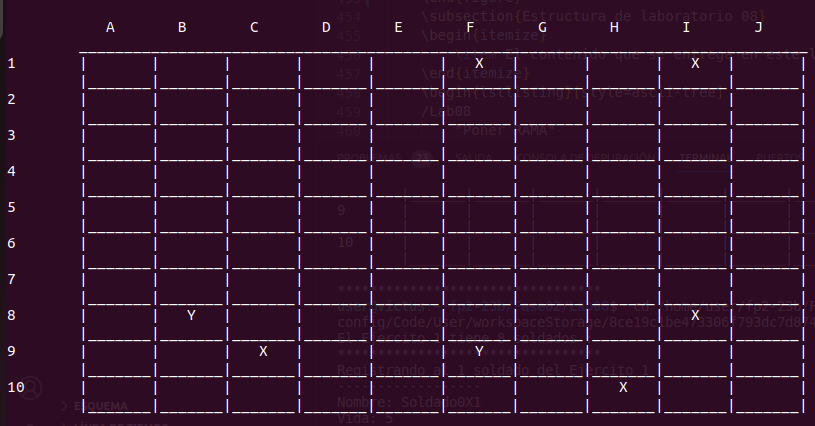
\includegraphics[width=1.0\textwidth,keepaspectratio]{img/Commit3.png}
		%\includesvg{img/automata.svg}
		%\label{img:mot2}
		%\caption{Product backlog.}
	\end{figure}
	\subsection{Ejercicio VideoJuego5}
	\begin{itemize}	
		\item En el cuarto commit modificamos el metodo viewBoard() en este haremos comparaciones entre los 2 ejercitos debido que en este podemos ver que 1 soldado de cada ejercito se puede cruzar debido a esto haremos una comprobacion de estos soldado de quien tienie mas vida para que se que de con ese casillero para eso va a ver una batalla la cual el ganador saldra con menos vida debido a la batalla y ganara el casillero para esto usamos bastantes if para comprobar esta situacion y vamos iterando por cada casillero para ver cada caso
		\item El codigo , el commit y la ejecucion seria el siguiente:
	\end{itemize}	
	\begin{lstlisting}[language=bash,caption={Commit}][H]
		$ git commit -m "Arreglando el tablero con las posiciones de cada bando de cada ejercito en caso de que soldados de diferente ejercito se encuentren en el mismo casillero estos van a tener una batalla como vemos en la que se compara su nivel de vida y el que tenga mas vida se posicionara donde esta siendo este el ganador pero su vida se reducira debido laa batalla tenida con el otro soldado el cual va a ser eliminado del campo"
	\end{lstlisting}	
	\begin{lstlisting}[language=java,caption={Las lineas de codigos del metodo creado:}][H]
		public static void viewBoard(HashMap<String, Soldado> army1, HashMap<String, Soldado> army2){ //EN ESTE METODO DEMOSTRAREMOS LA TABLA REUTILIZAREMOS CODIGOS DE ANTERIORES LABORATORIOS PARA PODER HACER LA BASE DE ESTE TABLERO
			System.out.println("\nMostrando tabla de posicion ... --");
			System.out.println("Leyenda: Ejercito1 --> X | Ejercito2 --> Y"); //RECONOCIMIENTO PARA LOS EJERCITOS Y POSICION DE SUS SOLDADOS
			System.out.println("\n \t   A\t   B\t   C\t   D\t   E\t   F\t   G\t   H\t   I\t   J"); // RECONOCIMIENTO PARA CADA UBICACION DE CADA SOLDADO EN EL TABLERO POR PARTE DE LAS COLUMNAS
			System.out.println("\t_________________________________________________________________________________");
			for(int i = 0; i < 10; i++ ){
				System.out.print((i + 1) + "\t"); // RECONOCIMIENTO PARA CADA UBICACION DE CADA SOLDADO EN EL TABLERO POR PARTE DE LAS FILAS
					for(int j = 0; j < 10; j++){
							if(army1.get("Soldado" + i + "X" + j) != null && army2.get("Soldado" + i + "X" + j) != null){ //CREAMOS UN IF PARA QUE ESTE NOS AYUDE A SABER QUIEN DE ESTOS SOLDADOS SE OCUPARA DEL CASILLERO EL CUAL DONDE ESTAN PELEANDO
								if(army1.get("Soldado" + i + "X" + j).getHealth() > army2.get("Soldado" + i + "X" + j).getHealth()){
									army1.get("Soldado" + i + "X" + j).setHealth(army1.get("Soldado" + i + "X" + j).getHealth() - army2.get("Soldado" + i + "X" + j).getHealth());
									army2.remove("Soldado" + i + "X" + j);
									System.out.print("|   " + "X" + "   ");
								}else if(army2.get("Soldado" + i + "X" + j) != null && army1.get("Soldado" + i + "X" + j) != null){
									army2.get("Soldado" + i + "X" + j).setHealth(army2.get("Soldado" + i + "X" + j).getHealth() - army1.get("Soldado" + i + "X" + j).getHealth());
									army1.remove("Soldado" + i + "X" + j);
									System.out.print("|   " + "Y" + "   ");
								}else{
									army2.remove("Soldado" + i + "X" + j);
									army1.remove("Soldado" + i + "X" + j);
									System.out.print("|   " + " " + "   ");
								}
							}else if(army1.get("Soldado" + i + "X" + j) != null){
								System.out.print("|   " + "X" + "   ");
							}else if(army2.get("Soldado" + i + "X" + j) != null){
								System.out.print("|   " + "Y" + "   ");
							}else{
								System.out.print("|   " + " " + "   ");
							}
					}
					System.out.println("|");
					System.out.println("\t|_______|_______|_______|_______|_______|_______|_______|_______|_______|_______|");
			}
			System.out.println("\n*********************************");
		
		}
		\end{lstlisting}
	\begin{lstlisting}[language=bash,caption={Ejecucion:}][H]
		El Ejercito 1 tiene 4 soldados : 
		*********************************
		Registrando al 1 soldado del Ejercito 1
		------------------
		Nombre: Soldado0X1
		Vida: 5
		Fila: 6
		Columna: J
		Registrando al 2 soldado del Ejercito 1
		------------------
		Nombre: Soldado1X1
		Vida: 4
		Fila: 7
		Columna: C
		Registrando al 3 soldado del Ejercito 1
		------------------
		Nombre: Soldado2X1
		Vida: 1
		Fila: 3
		Columna: A
		Registrando al 4 soldado del Ejercito 1
		------------------
		Nombre: Soldado3X1
		Vida: 5
		Fila: 2
		Columna: D
		El Ejercito 2 tiene 4 soldados : 
		*********************************
		Registrando al 1 soldado del Ejercito 2
		------------------
		Nombre: Soldado0X2
		Vida: 5
		Fila: 2
		Columna: J
		Registrando al 2 soldado del Ejercito 2
		------------------
		Nombre: Soldado1X2
		Vida: 1
		Fila: 7
		Columna: J
		Registrando al 3 soldado del Ejercito 2
		------------------
		Nombre: Soldado2X2
		Vida: 1
		Fila: 9
		Columna: B
		Registrando al 4 soldado del Ejercito 2
		------------------
		Nombre: Soldado3X2
		Vida: 2
		Fila: 6
		Columna: J
		
		Mostrando tabla de posicion ... --
		Leyenda: Ejercito1 --> X | Ejercito2 --> Y

	\end{lstlisting}
	\begin{figure}[H]
		\centering
		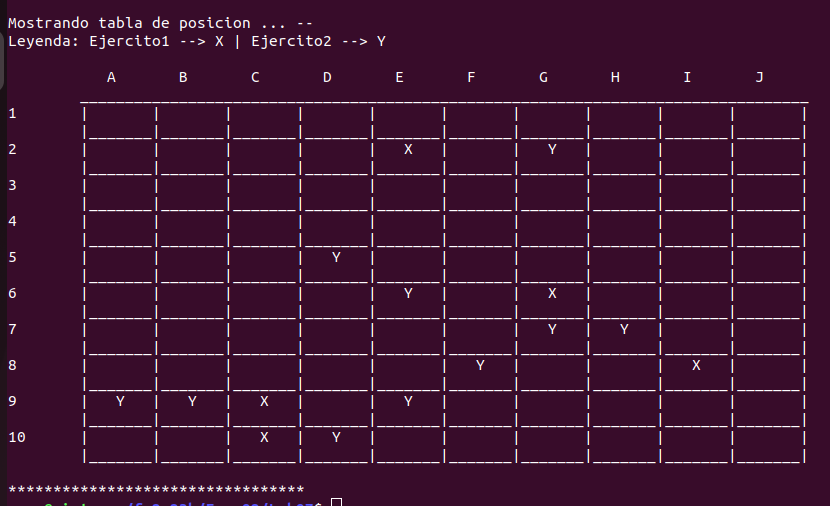
\includegraphics[width=1.0\textwidth,keepaspectratio]{img/Commit4.png}
		%\includesvg{img/automata.svg}
		%\label{img:mot2}
		%\caption{Product backlog.}
	\end{figure}
	\subsection{Ejercicio VideoJuego5}
	\begin{itemize}	
		\item En el quinto commit creamos el metodo longerLife() el cual nos podra a dar la informacion del soldado el cual tenga la mayor vida este se va comparando con otros soldados el cual tendra que hacer una iteracion con cada soldado de cada ejercito a la vez con esto comprobamos que el soldado el cual estamos buscando no sea nulo
		\item El codigo , el commit y la ejecucion seria el siguiente:
	\end{itemize}	
	\begin{lstlisting}[language=bash,caption={Commit}][H]
		$ git commit -m "Creamos el metodo longerLife() el cual nos podra a dar la informacion del soldado el cual tenga la mayor vida este se va comparando con otros soldados el cual tendra que hacer una iteracion con cada soldado de cada ejercito a la vez con esto comprobamos que el soldado el cual estamos buscando no sea nulo"
	\end{lstlisting}	
	\begin{lstlisting}[language=java,caption={Las lineas de codigos del metodo creado:}][H]
		public static void longerLife(HashMap<String, Soldado> army , int num){
			int mayor = 0;
			Soldado soldier = null;
			for(int i = 0; i < 10; i++){
				for(int j = 0; j < 10; j++){ //ITERACION LA CUAL NOS AYUDA A PASAR POR TODOS LOS SOLDADOS DE CADA EJERCITO
					if(army.get("Soldado" + i + "X" + j) != null){ //VERIFICAMOS QUE EL SOLDADO EL CUAL ESTAMOS VERIFICANOD NO SEA UNO NULO
						if(army.get("Soldado" + i + "X" + j).getHealth() > mayor){
							mayor = army.get("Soldado" + i + "X" + j).getHealth(); //DETECTAMOS EL MAYOR EL CUAL VAMOS COMPRANDO CON LOS DEMAS SOLDADOS PARA TENER SOLO AL SOLDADO EL CUAL TENGA LA MAYOR VIDA
							soldier = army.get("Soldado" + i + "X" + j); //SOLDIER CONTENDRA A ESTE SOLDADO EL CUAL DESPUES SE IMPRIMIRA SUS DATOS PARA VER DE QUE SOLDADO SE TRATA
						}
					}
				}
			}
			System.out.println("");
			System.out.println("El soldado con mayor vida del Ejercito " + num + " es: ");
			System.out.println(soldier.toString());
			System.out.println("*********************************");
		}
	\end{lstlisting}
	\begin{lstlisting}[language=bash,caption={Ejecucion:}][H]
		El Ejercito 1 tiene 7 soldados : 
		*********************************
		Registrando al 1 soldado del Ejercito 1
		------------------
		Nombre: Soldado0X1
		Vida: 5
		Fila: 9
		Columna: I
		Registrando al 2 soldado del Ejercito 1
		------------------
		Nombre: Soldado1X1
		Vida: 1
		Fila: 3
		Columna: D
		Registrando al 3 soldado del Ejercito 1
		------------------
		Nombre: Soldado2X1
		Vida: 5
		Fila: 9
		Columna: E
		Registrando al 4 soldado del Ejercito 1
		------------------
		Nombre: Soldado3X1
		Vida: 5
		Fila: 4
		Columna: G
		Registrando al 5 soldado del Ejercito 1
		------------------
		Nombre: Soldado4X1
		Vida: 4
		Fila: 3
		Columna: C
		Registrando al 6 soldado del Ejercito 1
		------------------
		Nombre: Soldado5X1
		Vida: 1
		Fila: 2
		Columna: C
		Registrando al 7 soldado del Ejercito 1
		------------------
		Nombre: Soldado6X1
		Vida: 3
		Fila: 10
		Columna: J
		El Ejercito 2 tiene 9 soldados : 
		*********************************
		Registrando al 1 soldado del Ejercito 2
		------------------
		Nombre: Soldado0X2
		Vida: 3
		Fila: 1
		Columna: H
		Registrando al 2 soldado del Ejercito 2
		------------------
		Nombre: Soldado1X2
		Vida: 3
		Fila: 2
		Columna: A
		Registrando al 3 soldado del Ejercito 2
		------------------
		Nombre: Soldado2X2
		Vida: 4
		Fila: 10
		Columna: G
		Registrando al 4 soldado del Ejercito 2
		------------------
		Nombre: Soldado3X2
		Vida: 3
		Fila: 9
		Columna: H
		Registrando al 5 soldado del Ejercito 2
		------------------
		Nombre: Soldado4X2
		Vida: 4
		Fila: 6
		Columna: H
		Registrando al 6 soldado del Ejercito 2
		------------------
		Nombre: Soldado5X2
		Vida: 4
		Fila: 9
		Columna: F
		Registrando al 7 soldado del Ejercito 2
		------------------
		Nombre: Soldado6X2
		Vida: 4
		Fila: 4
		Columna: A
		Registrando al 8 soldado del Ejercito 2
		------------------
		Nombre: Soldado7X2
		Vida: 2
		Fila: 9
		Columna: E
		Registrando al 9 soldado del Ejercito 2
		------------------
		Nombre: Soldado8X2
		Vida: 5
		Fila: 6
		Columna: J
		
		Mostrando tabla de posicion ... --
		Leyenda: Ejercito1 --> X | Ejercito2 --> Y		

	\end{lstlisting}
	\begin{figure}[H]
		\centering
		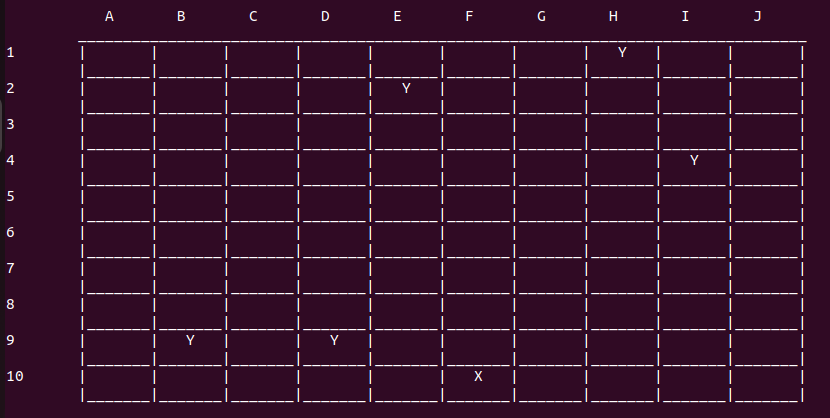
\includegraphics[width=1.0\textwidth,keepaspectratio]{img/Commit5.png}
		%\includesvg{img/automata.svg}
		%\label{img:mot2}
		%\caption{Product backlog.}
	\end{figure}
	\begin{lstlisting}[language=bash,caption={Ejecucion:}][H]
		*********************************

		El soldado con mayor vida del Ejercito 1 es: 

		Nombre: Soldado3X1
		Vida: 5
		Fila: 4
		Columna: G
		*********************************

		El soldado con mayor vida del Ejercito 2 es: 

		Nombre: Soldado8X2
		Vida: 5
		Fila: 6
		Columna: J
		*********************************

	\end{lstlisting}
	\subsection{Ejercicio VideoJuego5}
	\begin{itemize}	
		\item En el sexto commit creamos el metodo averageLife() en este metodo recolectamos la vida de cada uno de los soldados de un ejercito el cual se va recolectando para despues dividirlo entre la cantidad de soldados que hay en el ejercito esto nos devolvera este promedio el cual tambien se publica para el conocimiento del usuario
		\item El codigo , el commit y la ejecucion seria el siguiente:
	\end{itemize}	
	\begin{lstlisting}[language=bash,caption={Commit}][H]
		$ git commit -m "Creando el metodo averageLife() en este metodo recolectamos la vida de cada uno de los soldados de un ejercito el cual se va recolectando para despues dividirlo entre la cantidad de soldados que hay en el ejercito esto nos devolvera este promedio el cual tambien se publica para el conocimiento del usuario"
	\end{lstlisting}	
	\begin{lstlisting}[language=java,caption={Las lineas de codigos del metodo creado:}][H]
		public static double averageLife(HashMap<String, Soldado> army , int num){
			int sum = 0;
			int count = 0;
			Soldado soldier = null;
			System.out.println("El promedio de puntos de vida del Ejercito " + num + " es: ");
			for(int i = 0; i < 10; i++){
				for(int j = 0; j < 10; j++){ //ITERACION LA CUAL NOS AYUDA A PASAR POR TODOS LOS SOLDADOS DE CADA EJERCITO
					if(army.get("Soldado" + i + "X" + j) != null){ 
						sum += army.get("Soldado" + i + "X" + j).getHealth();
						count++;
					}
				}
			}
			if(sum != 0){
				double avg = sum / (count * 1.0);
				System.out.println(avg); // DAMOS A CONOCER EL PROMEDIO DE VIDA DE CADA EJERCITO 
				System.out.println("*********************************");
				return avg;
			}else{
				double avg = 0;
				System.out.println(avg); // DAMOS A CONOCER EL PROMEDIO DE VIDA DE CADA EJERCITO 
				System.out.println("*********************************");
				return avg;
			}
		}
	\end{lstlisting}
	\begin{lstlisting}[language=bash,caption={Ejecucion:}][H]
		El Ejercito 1 tiene 2 soldados : 
		*********************************
		Registrando al 1 soldado del Ejercito 1
		------------------
		Nombre: Soldado0X1
		Vida: 3
		Fila: 3
		Columna: G
		Registrando al 2 soldado del Ejercito 1
		------------------
		Nombre: Soldado1X1
		Vida: 2
		Fila: 9
		Columna: A
		El Ejercito 2 tiene 7 soldados : 
		*********************************
		Registrando al 1 soldado del Ejercito 2
		------------------
		Nombre: Soldado0X2
		Vida: 5
		Fila: 10
		Columna: D
		Registrando al 2 soldado del Ejercito 2
		------------------
		Nombre: Soldado1X2
		Vida: 4
		Fila: 6
		Columna: E
		Registrando al 3 soldado del Ejercito 2
		------------------
		Nombre: Soldado2X2
		Vida: 3
		Fila: 2
		Columna: H
		Registrando al 4 soldado del Ejercito 2
		------------------
		Nombre: Soldado3X2
		Vida: 5
		Fila: 8
		Columna: G
		Registrando al 5 soldado del Ejercito 2
		------------------
		Nombre: Soldado4X2
		Vida: 1
		Fila: 2
		Columna: D
		Registrando al 6 soldado del Ejercito 2
		------------------
		Nombre: Soldado5X2
		Vida: 2
		Fila: 2
		Columna: C
		Registrando al 7 soldado del Ejercito 2
		------------------
		Nombre: Soldado6X2
		Vida: 4
		Fila: 4
		Columna: A
		
		Mostrando tabla de posicion ... --
		Leyenda: Ejercito1 --> X | Ejercito2 --> Y
		
	\end{lstlisting}
	\begin{figure}[H]
		\centering
		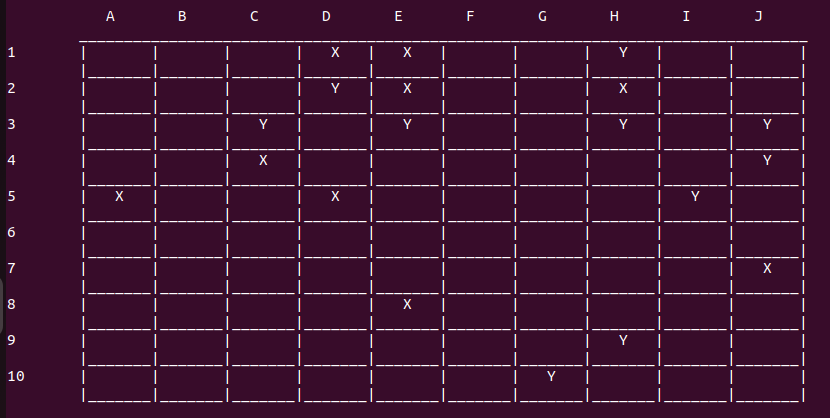
\includegraphics[width=1.0\textwidth,keepaspectratio]{img/Commit6.png}
		%\includesvg{img/automata.svg}
		%\label{img:mot2}
		%\caption{Product backlog.}
	\end{figure}
	\begin{lstlisting}[language=bash,caption={Ejecucion:}][H]
		*********************************

		El soldado con mayor vida del Ejercito 1 es: 
		
		Nombre: Soldado0X1
		Vida: 3
		Fila: 3
		Columna: G
		*********************************
		
		El soldado con mayor vida del Ejercito 2 es: 
		
		Nombre: Soldado3X2
		Vida: 5
		Fila: 8
		Columna: G
		*********************************
		El promedio de puntos de vida del Ejercito 1 es: 
		2.5
		*********************************
		El promedio de puntos de vida del Ejercito 2 es: 
		3.4285714285714284
		*********************************
		
	\end{lstlisting}
	\subsection{Ejercicio VideoJuego5}
	\begin{itemize}	
		\item En el septimo commit creamos el metodo rankingBurbujaLife() el cual nos ayuda a ordenar estos soldados de cada ejercito mediante su vida la cual para esto el HashMap su contenido lo pasamos a un array el cual este nos posibilita a que este metodo burubuja sea mas facil de intercambiar para despues imprimir al ejercito con sus respectivos puestos y soldados con su iformacion correspondiente para esto iterariamos cada elemento de este HashMap
		\item El codigo , el commit y la ejecucion seria el siguiente:
	\end{itemize}	
	\begin{lstlisting}[language=bash,caption={Commit}][H]
		$ git commit -m "Creamos el metodo rankingBurbujaLife() el cual nos ayuda a ordenar estos soldados de cada ejercito mediante su vida la cual para esto el HashMap su contenido lo pasamos a un array el cual este nos posibilita a que este metodo burubuja sea mas facil de intercambiar para despues imprimir al ejercito con sus respectivos puestos y soldados con su iformacion correspondiente para esto iterariamos cada elemento de este HashMap"
	\end{lstlisting}	
	\begin{lstlisting}[language=java,caption={Las lineas de codigos del metodo creado:}][H]
		public static void rankingBurbujaLife(HashMap<String, Soldado> army , int num){
			System.out.println("El Ejercito " + num + " ordenando por metodo burbuja: ");
			int count = 0;
			for(int i = 0; i < 10; i++){
				for(int j = 0; j < 10; j++){ //ITERACION LA CUAL NOS AYUDA A PASAR POR TODOS LOS SOLDADOS DE CADA EJERCITO
					if(army.get("Soldado" + i + "X" + j) != null){ 
					   count++;
					}
				}
			}
			System.out.println("------------------------------------------");
			System.out.println("Mostrando Ranking del Ejercito " + num + " ..... ////// --->");
			Soldado[] soldados = new Soldado[count];
			int x = 0;
			for(int i = 0; i < 10; i++){
				for(int j = 0; j < 10; j++){ //ITERACION LA CUAL NOS AYUDA A PASAR POR TODOS LOS SOLDADOS AL ARRAY SOLDADO PARA PODER USAR EL USO DEL METODO DE ORDENACION BURBUJA
					if(army.get("Soldado" + i + "X" + j) != null){ 
						if(count - count + x == count){
							break;
						}else{
							soldados[count - count + x] = army.get("Soldado" + i + "X" + j);
						}
						x++;   
					}
				}
			}
			int n = soldados.length;
			for (int i = 0; i < n - 1; i++) {
				for (int j = 0; j < n - 1 - i; j++) {
					if (soldados[j].getHealth() < soldados[j + 1].getHealth()) {
						// Intercambiar elementos si estan en el orden incorrecto
						Soldado temp = soldados[j];
						soldados[j] = soldados[j + 1];
						soldados[j + 1] = temp;
					}
				}
			}
			for(int i = 0; i < soldados.length; i++){
				System.out.print("\n" + "Puesto " + (i + 1));
				System.out.println(soldados[i].toString());
				System.out.println("------------------");
			}
			System.out.println("*********************************");
		}
	\end{lstlisting}
	\begin{lstlisting}[language=bash,caption={Ejecucion:}][H]
		El Ejercito 1 tiene 9 soldados : 
		*********************************
		Registrando al 1 soldado del Ejercito 1
		------------------
		Nombre: Soldado0X1
		Vida: 1
		Fila: 10
		Columna: D
		Registrando al 2 soldado del Ejercito 1
		------------------
		Nombre: Soldado1X1
		Vida: 5
		Fila: 10
		Columna: E
		Registrando al 3 soldado del Ejercito 1
		------------------
		Nombre: Soldado2X1
		Vida: 4
		Fila: 10
		Columna: F
		Registrando al 4 soldado del Ejercito 1
		------------------
		Nombre: Soldado3X1
		Vida: 4
		Fila: 7
		Columna: B
		Registrando al 5 soldado del Ejercito 1
		------------------
		Nombre: Soldado4X1
		Vida: 5
		Fila: 8
		Columna: D
		Registrando al 6 soldado del Ejercito 1
		------------------
		Nombre: Soldado5X1
		Vida: 1
		Fila: 3
		Columna: E
		Registrando al 7 soldado del Ejercito 1
		------------------
		Nombre: Soldado6X1
		Vida: 1
		Fila: 6
		Columna: G
		Registrando al 8 soldado del Ejercito 1
		------------------
		Nombre: Soldado7X1
		Vida: 1
		Fila: 3
		Columna: D
		Registrando al 9 soldado del Ejercito 1
		------------------
		Nombre: Soldado8X1
		Vida: 3
		Fila: 10
		Columna: G
		El Ejercito 2 tiene 7 soldados : 
		*********************************
		Registrando al 1 soldado del Ejercito 2
		------------------
		Nombre: Soldado0X2
		Vida: 1
		Fila: 3
		Columna: I
		Registrando al 2 soldado del Ejercito 2
		------------------
		Nombre: Soldado1X2
		Vida: 1
		Fila: 6
		Columna: I
		Registrando al 3 soldado del Ejercito 2
		------------------
		Nombre: Soldado2X2
		Vida: 4
		Fila: 6
		Columna: D
		Registrando al 4 soldado del Ejercito 2
		------------------
		Nombre: Soldado3X2
		Vida: 1
		Fila: 9
		Columna: D
		Registrando al 5 soldado del Ejercito 2
		------------------
		Nombre: Soldado4X2
		Vida: 4
		Fila: 9
		Columna: I
		Registrando al 6 soldado del Ejercito 2
		------------------
		Nombre: Soldado5X2
		Vida: 1
		Fila: 1
		Columna: A
		Registrando al 7 soldado del Ejercito 2
		------------------
		Nombre: Soldado6X2
		Vida: 3
		Fila: 1
		Columna: H
		
		Mostrando tabla de posicion ... --
		Leyenda: Ejercito1 --> X | Ejercito2 --> Y
			
	\end{lstlisting}
	\begin{figure}[H]
		\centering
		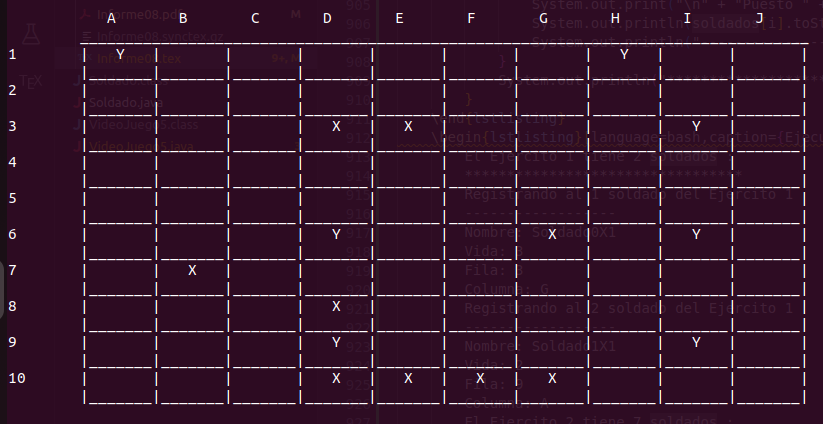
\includegraphics[width=1.0\textwidth,keepaspectratio]{img/Commit7.png}
		%\includesvg{img/automata.svg}
		%\label{img:mot2}
		%\caption{Product backlog.}
	\end{figure}
	\begin{lstlisting}[language=bash,caption={Ejecucion:}][H]
		*********************************

		El soldado con mayor vida del Ejercito 1 es: 
		
		Nombre: Soldado4X1
		Vida: 5
		Fila: 8
		Columna: D
		*********************************
		
		El soldado con mayor vida del Ejercito 2 es: 
		
		Nombre: Soldado2X2
		Vida: 4
		Fila: 6
		Columna: D
		*********************************
		El promedio de puntos de vida del Ejercito 1 es: 
		2.7777777777777777
		*********************************
		El promedio de puntos de vida del Ejercito 2 es: 
		2.142857142857143
		*********************************
		El Ejercito 1 ordenando por metodo burbuja: 
		------------------------------------------
		Mostrando Ranking del Ejercito 1 ..... ////// --->
		
		Puesto 1
		Nombre: Soldado4X1
		Vida: 5
		Fila: 8
		Columna: D
		------------------
		
		Puesto 2
		Nombre: Soldado1X1
		Vida: 5
		Fila: 10
		Columna: E
		------------------
		
		Puesto 3
		Nombre: Soldado3X1
		Vida: 4
		Fila: 7
		Columna: B
		------------------
		
		Puesto 4
		Nombre: Soldado2X1
		Vida: 4
		Fila: 10
		Columna: F
		------------------
		
		Puesto 5
		Nombre: Soldado8X1
		Vida: 3
		Fila: 10
		Columna: G
		------------------
		
		Puesto 6
		Nombre: Soldado7X1
		Vida: 1
		Fila: 3
		Columna: D
		------------------
		
		Puesto 7
		Nombre: Soldado5X1
		Vida: 1
		Fila: 3
		Columna: E
		------------------
		
		Puesto 8
		Nombre: Soldado6X1
		Vida: 1
		Fila: 6
		Columna: G
		------------------
		
		Puesto 9
		Nombre: Soldado0X1
		Vida: 1
		Fila: 10
		Columna: D
		------------------
		*********************************
		El Ejercito 2 ordenando por metodo burbuja: 
		------------------------------------------
		Mostrando Ranking del Ejercito 2 ..... ////// --->
		
		Puesto 1
		Nombre: Soldado2X2
		Vida: 4
		Fila: 6
		Columna: D
		------------------
		
		Puesto 2
		Nombre: Soldado4X2
		Vida: 4
		Fila: 9
		Columna: I
		------------------
		
		Puesto 3
		Nombre: Soldado6X2
		Vida: 3
		Fila: 1
		Columna: H
		------------------
		
		Puesto 4
		Nombre: Soldado5X2
		Vida: 1
		Fila: 1
		Columna: A
		------------------
		
		Puesto 5
		Nombre: Soldado0X2
		Vida: 1
		Fila: 3
		Columna: I
		------------------
		
		Puesto 6
		Nombre: Soldado1X2
		Vida: 1
		Fila: 6
		Columna: I
		------------------
		
		Puesto 7
		Nombre: Soldado3X2
		Vida: 1
		Fila: 9
		Columna: D
		------------------
		*********************************
		
	\end{lstlisting}
	\subsection{Ejercicio VideoJuego5}
	\begin{itemize}	
		\item En el octavo commit creamos el metodo rankingInsercionLife() el cual nos ayuda a ordenar a los soldados pero esta ves de forma inserciva la cual tendria la misma logica que el anterior metodo pero este se aplicaria diferente ya que este tendria su propia funcionalidad la cual la hace unica y despues de esto podemos publicar resultados de cada ejercito el cual va del mayor al menor
		\item El codigo , el commit y la ejecucion seria el siguiente:
	\end{itemize}	
	\begin{lstlisting}[language=bash,caption={Commit}][H]
		$ git commit -m "Creamos el metodo rankingInsercionLife() el cual nos ayuda a ordenar a los soldados pero esta ves de forma inserciva la cual tendria la misma logica que el anterior metodo pero este se aplicaria diferente ya que este tendria su propia funcionalidad la cual la hace unica y despues de esto podemos publicar resultados de cada ejercito el cual va del mayor al menor"
	\end{lstlisting}	
	\begin{lstlisting}[language=java,caption={Las lineas de codigos del metodo creado:}][H]
		public static void rankingInsercionLife(HashMap<String, Soldado> army , int num){
			System.out.println("El Ejercito " + num + " ordenando por metodo insercion: ");
			int count = 0;
			for(int i = 0; i < 10; i++){
				for(int j = 0; j < 10; j++){ //ITERACION LA CUAL NOS AYUDA A PASAR POR TODOS LOS SOLDADOS DE CADA EJERCITO
					if(army.get("Soldado" + i + "X" + j) != null){ 
					   count++;
					}
				}
			}
			System.out.println("------------------------------------------");
			System.out.println("Mostrando Ranking del Ejercito " + num + " ..... ////// --->");
			Soldado[] soldados = new Soldado[count];
			int x = 0;
			for(int i = 0; i < 10; i++){
				for(int j = 0; j < 10; j++){ //ITERACION LA CUAL NOS AYUDA A PASAR POR TODOS LOS SOLDADOS AL ARRAY SOLDADO PARA PODER USAR EL USO DEL METODO DE ORDENACION INSERCION
					if(army.get("Soldado" + i + "X" + j) != null){ 
						if(count - count + x == count){
							break;
						}else{
							soldados[count - count + x] = army.get("Soldado" + i + "X" + j); //LA MISMA LOGICA QUE EL ANTERIOR METODO SOLO QUE EN ESTE LO USARIAMOS DE MANERA DIFERENTE YA QUE ESTE SERIA DE FORMA DE INSERCION
						}
						x++;   
					}
				}
			}
			int n = soldados.length;
			for (int i = 1; i < n; i++) {
				Soldado actual = soldados[i];
				int j = i - 1;
				while (j >= 0 && soldados[j].getHealth() < actual.getHealth()) { //ORDENAMOS EL EJERCITO RESPECTIVAMENTE MEDIANTE EL METODO QUE NOS OFRECE INSERCION EL CUAL ES ESTE CODIGO
					soldados[j + 1] = soldados[j];
					j--;
				}
				soldados[j + 1] = actual;
			}
			for(int i = 0; i < soldados.length; i++){
				System.out.print("\n" + "Puesto " + (i + 1));
				System.out.println(soldados[i].toString()); //PUBLICAMOS RESULTADOS
				System.out.println("------------------");
			}
			System.out.println("*********************************");
		}
	\end{lstlisting}
	\begin{lstlisting}[language=bash,caption={Ejecucion:}][H]
		El Ejercito 1 tiene 1 soldados : 
		*********************************
		Registrando al 1 soldado del Ejercito 1
		------------------
		Nombre: Soldado0X1
		Vida: 3
		Fila: 5
		Columna: D
		El Ejercito 2 tiene 1 soldados : 
		*********************************
		Registrando al 1 soldado del Ejercito 2
		------------------
		Nombre: Soldado0X2
		Vida: 3
		Fila: 4
		Columna: C

		Mostrando tabla de posicion ... --
		Leyenda: Ejercito1 --> X | Ejercito2 --> Y

	\end{lstlisting}
	\begin{figure}[H]
		\centering
		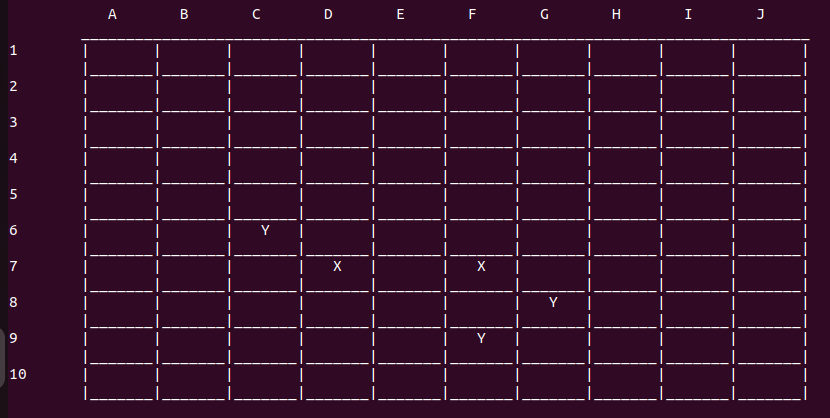
\includegraphics[width=1.0\textwidth,keepaspectratio]{img/Commit8.png}
		%\includesvg{img/automata.svg}
		%\label{img:mot2}
		%\caption{Product backlog.}
	\end{figure}
	\begin{lstlisting}[language=bash,caption={Ejecucion:}][H]
		*********************************

		El soldado con mayor vida del Ejercito 1 es: 
		
		Nombre: Soldado0X1
		Vida: 3
		Fila: 5
		Columna: D
		*********************************
		
		El soldado con mayor vida del Ejercito 2 es: 
		
		Nombre: Soldado0X2
		Vida: 3
		Fila: 4
		Columna: C
		*********************************
		El promedio de puntos de vida del Ejercito 1 es: 
		3.0
		*********************************
		El promedio de puntos de vida del Ejercito 2 es: 
		3.0
		*********************************
		El Ejercito 1 ordenando por metodo burbuja: 
		------------------------------------------
		Mostrando Ranking del Ejercito 1 ..... ////// --->
		
		Puesto 1
		Nombre: Soldado0X1
		Vida: 3
		Fila: 5
		Columna: D
		------------------
		*********************************
		El Ejercito 2 ordenando por metodo burbuja: 
		------------------------------------------
		Mostrando Ranking del Ejercito 2 ..... ////// --->
		
		Puesto 1
		Nombre: Soldado0X2
		Vida: 3
		Fila: 4
		Columna: C
		------------------
		*********************************
		El Ejercito 1 ordenando por metodo insercion: 
		------------------------------------------
		Mostrando Ranking del Ejercito 1 ..... ////// --->
		
		Puesto 1
		Nombre: Soldado0X1
		Vida: 3
		Fila: 5
		Columna: D
		------------------
		*********************************
		El Ejercito 2 ordenando por metodo insercion: 
		------------------------------------------
		Mostrando Ranking del Ejercito 2 ..... ////// --->
		
		Puesto 1
		Nombre: Soldado0X2
		Vida: 3
		Fila: 4
		Columna: C
		------------------
		*********************************
		
	\end{lstlisting}
	\subsection{Ejercicio VideoJuego5}
	\begin{itemize}	
		\item En el noveno commit creamos el metodo resultBattle() el cual nos dara el resultado de esta batalla dependiendo del promedio de estos 2 ejercitos debido a esto se va generar un ganador para esto se comparan estas 2 cantidades metodologia promedio de vida de cada ejercito
		\item El codigo , el commit y la ejecucion seria el siguiente:
	\end{itemize}	
	\begin{lstlisting}[language=bash,caption={Commit}][H]
		$ git commit -m "Creamos el metodo resultBattle() el cual nos dara el resultado de esta batalla dependiendo del promedio de estos 2 ejercitos debido a esto se va generar un ganador para esto se comparan estas 2 cantidades metodologia promedio de vida de cada ejercito"
	\end{lstlisting}	
	\begin{lstlisting}[language=java,caption={Las lineas de codigos del metodo creado:}][H]
		public static void resultBattle(double avg1, double avg2,  int num, int num2){ //METODO CREADO PARA PODER SABER EL RESULTADO DE ESTA BATALLA ENTRE ESTOS 2 EJERCITOS
			if(avg1 > avg2){ //PUBLICACION DE LOS RESULTADOS
				System.out.println("El Ejercito " + num + " es el GANADOR con " + avg1+ " puntos");
			}else if(avg2 > avg1){
				System.out.println("El Ejercito " + num2 + " es el GANADOR con " + avg2 + " puntos");
			}else{
				System.out.println("EMPATE con " + avg1 + " puntos");
			}
		}
	\end{lstlisting}
	\begin{lstlisting}[language=bash,caption={Ejecucion:}][H]
		El Ejercito 1 tiene 6 soldados : 
		*********************************
		Registrando al 1 soldado del Ejercito 1
		------------------
		Nombre: Soldado0X1
		Vida: 3
		Fila: 5
		Columna: J
		Registrando al 2 soldado del Ejercito 1
		------------------
		Nombre: Soldado1X1
		Vida: 5
		Fila: 2
		Columna: B
		Registrando al 3 soldado del Ejercito 1
		------------------
		Nombre: Soldado2X1
		Vida: 3
		Fila: 5
		Columna: G
		Registrando al 4 soldado del Ejercito 1
		------------------
		Nombre: Soldado3X1
		Vida: 2
		Fila: 1
		Columna: C
		Registrando al 5 soldado del Ejercito 1
		------------------
		Nombre: Soldado4X1
		Vida: 3
		Fila: 10
		Columna: H
		Registrando al 6 soldado del Ejercito 1
		------------------
		Nombre: Soldado5X1
		Vida: 4
		Fila: 10
		Columna: D
		El Ejercito 2 tiene 6 soldados : 
		*********************************
		Registrando al 1 soldado del Ejercito 2
		------------------
		Nombre: Soldado0X2
		Vida: 1
		Fila: 9
		Columna: D
		Registrando al 2 soldado del Ejercito 2
		------------------
		Nombre: Soldado1X2
		Vida: 3
		Fila: 5
		Columna: F
		Registrando al 3 soldado del Ejercito 2
		------------------
		Nombre: Soldado2X2
		Vida: 5
		Fila: 9
		Columna: G
		Registrando al 4 soldado del Ejercito 2
		------------------
		Nombre: Soldado3X2
		Vida: 3
		Fila: 10
		Columna: A
		Registrando al 5 soldado del Ejercito 2
		------------------
		Nombre: Soldado4X2
		Vida: 2
		Fila: 4
		Columna: F
		Registrando al 6 soldado del Ejercito 2
		------------------
		Nombre: Soldado5X2
		Vida: 4
		Fila: 10
		Columna: E
		
		Mostrando tabla de posicion ... --
		Leyenda: Ejercito1 --> X | Ejercito2 --> Y
		
	\end{lstlisting}
	\begin{figure}[H]
		\centering
		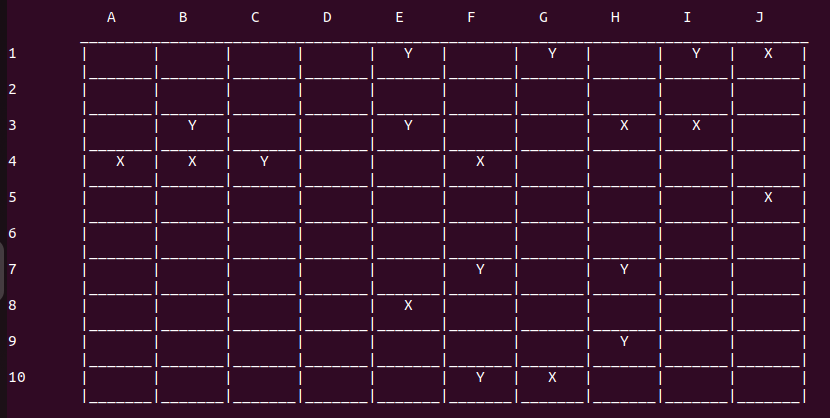
\includegraphics[width=1.0\textwidth,keepaspectratio]{img/Commit9.png}
		%\includesvg{img/automata.svg}
		%\label{img:mot2}
		%\caption{Product backlog.}
	\end{figure}
	\begin{lstlisting}[language=bash,caption={Ejecucion:}][H]
		*********************************

		El soldado con mayor vida del Ejercito 1 es: 
		
		Nombre: Soldado1X1
		Vida: 5
		Fila: 2
		Columna: B
		*********************************
		
		El soldado con mayor vida del Ejercito 2 es: 
		
		Nombre: Soldado2X2
		Vida: 5
		Fila: 9
		Columna: G
		*********************************
		El promedio de puntos de vida del Ejercito 1 es: 
		3.3333333333333335
		*********************************
		El promedio de puntos de vida del Ejercito 2 es: 
		3.0
		*********************************
		El Ejercito 1 ordenando por metodo burbuja: 
		------------------------------------------
		Mostrando Ranking del Ejercito 1 ..... ////// --->
		
		Puesto 1
		Nombre: Soldado1X1
		Vida: 5
		Fila: 2
		Columna: B
		------------------
		
		Puesto 2
		Nombre: Soldado5X1
		Vida: 4
		Fila: 10
		Columna: D
		------------------
		
		Puesto 3
		Nombre: Soldado2X1
		Vida: 3
		Fila: 5
		Columna: G
		------------------
		
		Puesto 4
		Nombre: Soldado0X1
		Vida: 3
		Fila: 5
		Columna: J
		------------------
		
		Puesto 5
		Nombre: Soldado4X1
		Vida: 3
		Fila: 10
		Columna: H
		------------------
		
		Puesto 6
		Nombre: Soldado3X1
		Vida: 2
		Fila: 1
		Columna: C
		------------------
		*********************************
		El Ejercito 2 ordenando por metodo burbuja: 
		------------------------------------------
		Mostrando Ranking del Ejercito 2 ..... ////// --->
		
		Puesto 1
		Nombre: Soldado2X2
		Vida: 5
		Fila: 9
		Columna: G
		------------------
		
		Puesto 2
		Nombre: Soldado5X2
		Vida: 4
		Fila: 10
		Columna: E
		------------------
		
		Puesto 3
		Nombre: Soldado1X2
		Vida: 3
		Fila: 5
		Columna: F
		------------------
		
		Puesto 4
		Nombre: Soldado3X2
		Vida: 3
		Fila: 10
		Columna: A
		------------------
		
		Puesto 5
		Nombre: Soldado4X2
		Vida: 2
		Fila: 4
		Columna: F
		------------------
		
		Puesto 6
		Nombre: Soldado0X2
		Vida: 1
		Fila: 9
		Columna: D
		------------------
		*********************************
		El Ejercito 1 ordenando por metodo insercion: 
		------------------------------------------
		Mostrando Ranking del Ejercito 1 ..... ////// --->
		
		Puesto 1
		Nombre: Soldado1X1
		Vida: 5
		Fila: 2
		Columna: B
		------------------
		
		Puesto 2
		Nombre: Soldado5X1
		Vida: 4
		Fila: 10
		Columna: D
		------------------
		
		Puesto 3
		Nombre: Soldado2X1
		Vida: 3
		Fila: 5
		Columna: G
		------------------
		
		Puesto 4
		Nombre: Soldado0X1
		Vida: 3
		Fila: 5
		Columna: J
		------------------
		
		Puesto 5
		Nombre: Soldado4X1
		Vida: 3
		Fila: 10
		Columna: H
		------------------
		
		Puesto 6
		Nombre: Soldado3X1
		Vida: 2
		Fila: 1
		Columna: C
		------------------
		*********************************
		El Ejercito 2 ordenando por metodo insercion: 
		------------------------------------------
		Mostrando Ranking del Ejercito 2 ..... ////// --->
		
		Puesto 1
		Nombre: Soldado2X2
		Vida: 5
		Fila: 9
		Columna: G
		------------------
		
		Puesto 2
		Nombre: Soldado5X2
		Vida: 4
		Fila: 10
		Columna: E
		------------------
		
		Puesto 3
		Nombre: Soldado1X2
		Vida: 3
		Fila: 5
		Columna: F
		------------------
		
		Puesto 4
		Nombre: Soldado3X2
		Vida: 3
		Fila: 10
		Columna: A
		------------------
		
		Puesto 5
		Nombre: Soldado4X2
		Vida: 2
		Fila: 4
		Columna: F
		------------------
		
		Puesto 6
		Nombre: Soldado0X2
		Vida: 1
		Fila: 9
		Columna: D
		------------------
		*********************************
		El Ejercito 1 es el GANADOR con 3.3333333333333335 puntos
		
	\end{lstlisting}
	\subsection{Ejercicio VideoJuego5}
	\begin{itemize}	
		\item En este apartado publicaremos el codigo completo y su ejecucion
		\item El codigo y la ejecucion seria el siguiente:
	\end{itemize}		
	\begin{lstlisting}[language=java,caption={Las lineas de codigos del metodo creado:}][H]
		// Laboratorio Nro 8  - Ejercicio VideoJuego5
		// Autor: Mamani Anahua Victor Narciso
		// Colaboro:
		// Tiempo:
		import java.util.*;
		class VideoJuego5{
			public static HashMap<String, Soldado> mapHashFillRegister(int num){
				Random rdm =new Random();
				HashMap<String, Soldado> army1 = new HashMap<String, Soldado>();
				ArrayList<ArrayList<Soldado>> army = new ArrayList<ArrayList<Soldado>>(); //NOS AYUDARIAMOS DE UN ARRAYLIST PARA PODER AYUDARNOS CON EL USO DE HASHMAPS PARA PODER REGISTAR A SOLDADOS EN LA QUE NINGUNO DE ESTOS SE REPITA 
				int numsoldiers = rdm.nextInt(10) + 1; //NUMERO DE SOLDADOS QUE SE VAN A CREAR DE 1 AL 10 
				for(int i = 0; i < 10; i++){
					army.add(new ArrayList<Soldado>()); //LLENAMOS NUESTROS ARRAYLIST BIDIMENSIONAL CON CADA FILA PARA QUE CUMPLAN CON ESTRUCTURA DEL TABLERO
					for(int j = 0; j < 10 ; j++){
						army.get(i).add(null); // LLENAMOS CADA FILA DEL ARRAYLIST CON UN OBJETO SOLDADO CON TAL QUE ESTE SEA NULL PARA QUE SEPA QUE ESTE TIENE UNA CASILLA PERO NO HAY NADIE TODAVIA SE PUEDE LLENAR 
						army1.put("Soldado" + i +"X" + j, null);
					}
				}
				System.out.println("El Ejercito " + num + " tiene " + numsoldiers + " soldados : " ); 
				System.out.println("*********************************");
				for(int i = 0; i < numsoldiers; i++){ //ITERACION PARA PODER DARLES LOS DATOS A CADA SOLDADO CREADO 
					String name = "Soldado" + i + "X" + num;
					int health = rdm.nextInt(5) + 1;
					int row = rdm.nextInt(10) + 1;
					String column = String.valueOf((char)(rdm.nextInt(10) + 65)); //REUTILIZAMOS CODIGO DEL ANTERIOR ARCHIVO VIDEOJUEGO4.JAVA YA QUE TENDRIAN LA MISMA FUNCIONALIDAD
					if(army.get(row - 1).get((int)column.charAt(0) - 65) == null){ 
						System.out.println("Registrando al " + (i + 1) + " soldado del Ejercito " + num + "");
						System.out.print("------------------");
						army.get(row - 1).set((int)column.charAt(0) - 65, new Soldado(name, health, row, column));
						army1.put("Soldado" + (row - 1) + "X" + ((int)(column.charAt(0)) - 65), new Soldado(name, health, row, column)); //INTEGRAMOS AL HASHMAP AL SOLDADO CON SU RESPECTIVO NOMBRE Y VALOR 
						System.out.println(army1.get("Soldado" + (row - 1) + "X" + ((int)(column.charAt(0)) - 65)).toString()); //PUBLICAMOS AL SOLDADO CREADO POR ORDEN DE CREACION
					}else{
						i -= 1; //NOS AYUDARIA CON LOS SOLDADOS QUE SE REPITEN EN EL MISMO CASILLERO CON TAL QUE NO DEBERIA CONTAR 
					}
				}
				return army1;
			}
			public static void viewBoard(HashMap<String, Soldado> army1, HashMap<String, Soldado> army2){ //EN ESTE METODO DEMOSTRAREMOS LA TABLA REUTILIZAREMOS CODIGOS DE ANTERIORES LABORATORIOS PARA PODER HACER LA BASE DE ESTE TABLERO
				System.out.println("\nMostrando tabla de posicion ... --");
				System.out.println("Leyenda: Ejercito1 --> X | Ejercito2 --> Y"); //RECONOCIMIENTO PARA LOS EJERCITOS Y POSICION DE SUS SOLDADOS
				System.out.println("\n \t   A\t   B\t   C\t   D\t   E\t   F\t   G\t   H\t   I\t   J"); // RECONOCIMIENTO PARA CADA UBICACION DE CADA SOLDADO EN EL TABLERO POR PARTE DE LAS COLUMNAS
				System.out.println("\t_________________________________________________________________________________");
				for(int i = 0; i < 10; i++ ){
					System.out.print((i + 1) + "\t"); // RECONOCIMIENTO PARA CADA UBICACION DE CADA SOLDADO EN EL TABLERO POR PARTE DE LAS FILAS
						for(int j = 0; j < 10; j++){
								if(army1.get("Soldado" + i + "X" + j) != null && army2.get("Soldado" + i + "X" + j) != null){ //CREAMOS UN IF PARA QUE ESTE NOS AYUDE A SABER QUIEN DE ESTOS SOLDADOS SE OCUPARA DEL CASILLERO EL CUAL DONDE ESTAN PELEANDO
									if(army1.get("Soldado" + i + "X" + j).getHealth() > army2.get("Soldado" + i + "X" + j).getHealth()){
										army1.get("Soldado" + i + "X" + j).setHealth(army1.get("Soldado" + i + "X" + j).getHealth() - army2.get("Soldado" + i + "X" + j).getHealth());
										army2.remove("Soldado" + i + "X" + j);
										System.out.print("|   " + "X" + "   ");
									}else if(army2.get("Soldado" + i + "X" + j) != null && army1.get("Soldado" + i + "X" + j) != null){
										army2.get("Soldado" + i + "X" + j).setHealth(army2.get("Soldado" + i + "X" + j).getHealth() - army1.get("Soldado" + i + "X" + j).getHealth());
										army1.remove("Soldado" + i + "X" + j);
										System.out.print("|   " + "Y" + "   ");
									}else{
										army2.remove("Soldado" + i + "X" + j);
										army1.remove("Soldado" + i + "X" + j);
										System.out.print("|   " + " " + "   ");
									}
								}else if(army1.get("Soldado" + i + "X" + j) != null){
									System.out.print("|   " + "X" + "   ");
								}else if(army2.get("Soldado" + i + "X" + j) != null){
									System.out.print("|   " + "Y" + "   ");
								}else{
									System.out.print("|   " + " " + "   ");
								}
						}
						System.out.println("|");
						System.out.println("\t|_______|_______|_______|_______|_______|_______|_______|_______|_______|_______|");
				}
				System.out.println("\n*********************************");
			
			}
			public static void longerLife(HashMap<String, Soldado> army , int num){
				int mayor = 0;
				Soldado soldier = null;
				for(int i = 0; i < 10; i++){
					for(int j = 0; j < 10; j++){ //ITERACION LA CUAL NOS AYUDA A PASAR POR TODOS LOS SOLDADOS DE CADA EJERCITO
						if(army.get("Soldado" + i + "X" + j) != null){ //VERIFICAMOS QUE EL SOLDADO EL CUAL ESTAMOS VERIFICANOD NO SEA UNO NULO
							if(army.get("Soldado" + i + "X" + j).getHealth() > mayor){
								mayor = army.get("Soldado" + i + "X" + j).getHealth(); //DETECTAMOS EL MAYOR EL CUAL VAMOS COMPRANDO CON LOS DEMAS SOLDADOS PARA TENER SOLO AL SOLDADO EL CUAL TENGA LA MAYOR VIDA
								soldier = army.get("Soldado" + i + "X" + j); //SOLDIER CONTENDRA A ESTE SOLDADO EL CUAL DESPUES SE IMPRIMIRA SUS DATOS PARA VER DE QUE SOLDADO SE TRATA
							}
						}
					}
				}
				System.out.println("");
				System.out.println("El soldado con mayor vida del Ejercito " + num + " es: ");
				System.out.println(soldier.toString());
				System.out.println("*********************************");
			}
			public static double averageLife(HashMap<String, Soldado> army , int num){
				int sum = 0;
				int count = 0;
				Soldado soldier = null;
				System.out.println("El promedio de puntos de vida del Ejercito " + num + " es: ");
				for(int i = 0; i < 10; i++){
					for(int j = 0; j < 10; j++){ //ITERACION LA CUAL NOS AYUDA A PASAR POR TODOS LOS SOLDADOS DE CADA EJERCITO
						if(army.get("Soldado" + i + "X" + j) != null){ 
							sum += army.get("Soldado" + i + "X" + j).getHealth();
							count++;
						}
					}
				}
				if(sum != 0){
					double avg = sum / (count * 1.0);
					System.out.println(avg); // DAMOS A CONOCER EL PROMEDIO DE VIDA DE CADA EJERCITO 
					System.out.println("*********************************");
					return avg;
				}else{
					double avg = 0;
					System.out.println(avg); // DAMOS A CONOCER EL PROMEDIO DE VIDA DE CADA EJERCITO 
					System.out.println("*********************************");
					return avg;
				}
			}
			public static void rankingBurbujaLife(HashMap<String, Soldado> army , int num){
				System.out.println("El Ejercito " + num + " ordenando por metodo burbuja: ");
				int count = 0;
				for(int i = 0; i < 10; i++){
					for(int j = 0; j < 10; j++){ //ITERACION LA CUAL NOS AYUDA A PASAR POR TODOS LOS SOLDADOS DE CADA EJERCITO
						if(army.get("Soldado" + i + "X" + j) != null){ 
						   count++;
						}
					}
				}
				System.out.println("------------------------------------------");
				System.out.println("Mostrando Ranking del Ejercito " + num + " ..... ////// --->");
				Soldado[] soldados = new Soldado[count];
				int x = 0;
				for(int i = 0; i < 10; i++){
					for(int j = 0; j < 10; j++){ //ITERACION LA CUAL NOS AYUDA A PASAR POR TODOS LOS SOLDADOS AL ARRAY SOLDADO PARA PODER USAR EL USO DEL METODO DE ORDENACION BURBUJA
						if(army.get("Soldado" + i + "X" + j) != null){ 
							if(count - count + x == count){
								break;
							}else{
								soldados[count - count + x] = army.get("Soldado" + i + "X" + j);
							}
							x++;   
						}
					}
				}
				int n = soldados.length;
				for (int i = 0; i < n - 1; i++) {
					for (int j = 0; j < n - 1 - i; j++) {
						if (soldados[j].getHealth() < soldados[j + 1].getHealth()) {
							// Intercambiar elementos si estan en el orden incorrecto
							Soldado temp = soldados[j];
							soldados[j] = soldados[j + 1];
							soldados[j + 1] = temp;
						}
					}
				}
				for(int i = 0; i < soldados.length; i++){
					System.out.print("\n" + "Puesto " + (i + 1));
					System.out.println(soldados[i].toString());
					System.out.println("------------------");
				}
				System.out.println("*********************************");
			}
			public static void rankingInsercionLife(HashMap<String, Soldado> army , int num){
				System.out.println("El Ejercito " + num + " ordenando por metodo insercion: ");
				int count = 0;
				for(int i = 0; i < 10; i++){
					for(int j = 0; j < 10; j++){ //ITERACION LA CUAL NOS AYUDA A PASAR POR TODOS LOS SOLDADOS DE CADA EJERCITO
						if(army.get("Soldado" + i + "X" + j) != null){ 
						   count++;
						}
					}
				}
				System.out.println("------------------------------------------");
				System.out.println("Mostrando Ranking del Ejercito " + num + " ..... ////// --->");
				Soldado[] soldados = new Soldado[count];
				int x = 0;
				for(int i = 0; i < 10; i++){
					for(int j = 0; j < 10; j++){ //ITERACION LA CUAL NOS AYUDA A PASAR POR TODOS LOS SOLDADOS AL ARRAY SOLDADO PARA PODER USAR EL USO DEL METODO DE ORDENACION INSERCION
						if(army.get("Soldado" + i + "X" + j) != null){ 
							if(count - count + x == count){
								break;
							}else{
								soldados[count - count + x] = army.get("Soldado" + i + "X" + j); //LA MISMA LOGICA QUE EL ANTERIOR METODO SOLO QUE EN ESTE LO USARIAMOS DE MANERA DIFERENTE YA QUE ESTE SERIA DE FORMA DE INSERCION
							}
							x++;   
						}
					}
				}
				int n = soldados.length;
				for (int i = 1; i < n; i++) {
					Soldado actual = soldados[i];
					int j = i - 1;
					while (j >= 0 && soldados[j].getHealth() < actual.getHealth()) { //ORDENAMOS EL EJERCITO RESPECTIVAMENTE MEDIANTE EL METODO QUE NOS OFRECE INSERCION EL CUAL ES ESTE CODIGO
						soldados[j + 1] = soldados[j];
						j--;
					}
					soldados[j + 1] = actual;
				}
				for(int i = 0; i < soldados.length; i++){
					System.out.print("\n" + "Puesto " + (i + 1));
					System.out.println(soldados[i].toString()); //PUBLICAMOS RESULTADOS
					System.out.println("------------------");
				}
				System.out.println("*********************************");
			}
			public static void resultBattle(double avg1, double avg2,  int num, int num2){ //METODO CREADO PARA PODER SABER EL RESULTADO DE ESTA BATALLA ENTRE ESTOS 2 EJERCITOS
				if(avg1 > avg2){ //PUBLICACION DE LOS RESULTADOS
					System.out.println("El Ejercito " + num + " es el GANADOR con " + avg1+ " puntos");
				}else if(avg2 > avg1){
					System.out.println("El Ejercito " + num2 + " es el GANADOR con " + avg2 + " puntos");
				}else{
					System.out.println("EMPATE con " + avg1 + " puntos");
				}
			}
			public static void main (String args []){
				HashMap<String, Soldado> army1 = mapHashFillRegister(1);
				HashMap<String, Soldado> army2 = mapHashFillRegister(2);
				viewBoard(army1, army2);
				longerLife(army1, 1);
				longerLife(army2, 2);
				double avgarmy1 = averageLife(army1, 1);
				double avgarmy2 = averageLife(army2, 2);
				rankingBurbujaLife(army1, 1);
				rankingBurbujaLife(army2, 2);
				rankingInsercionLife(army1, 1);
				rankingInsercionLife(army2, 2);
				resultBattle(avgarmy1, avgarmy2, 1, 2);
			}
		}
	\end{lstlisting}
	\begin{lstlisting}[language=bash,caption={Ejecucion:}][H]
		El Ejercito 1 tiene 6 soldados : 
		*********************************
		Registrando al 1 soldado del Ejercito 1
		------------------
		Nombre: Soldado0X1
		Vida: 3
		Fila: 5
		Columna: J
		Registrando al 2 soldado del Ejercito 1
		------------------
		Nombre: Soldado1X1
		Vida: 5
		Fila: 2
		Columna: B
		Registrando al 3 soldado del Ejercito 1
		------------------
		Nombre: Soldado2X1
		Vida: 3
		Fila: 5
		Columna: G
		Registrando al 4 soldado del Ejercito 1
		------------------
		Nombre: Soldado3X1
		Vida: 2
		Fila: 1
		Columna: C
		Registrando al 5 soldado del Ejercito 1
		------------------
		Nombre: Soldado4X1
		Vida: 3
		Fila: 10
		Columna: H
		Registrando al 6 soldado del Ejercito 1
		------------------
		Nombre: Soldado5X1
		Vida: 4
		Fila: 10
		Columna: D
		El Ejercito 2 tiene 6 soldados : 
		*********************************
		Registrando al 1 soldado del Ejercito 2
		------------------
		Nombre: Soldado0X2
		Vida: 1
		Fila: 9
		Columna: D
		Registrando al 2 soldado del Ejercito 2
		------------------
		Nombre: Soldado1X2
		Vida: 3
		Fila: 5
		Columna: F
		Registrando al 3 soldado del Ejercito 2
		------------------
		Nombre: Soldado2X2
		Vida: 5
		Fila: 9
		Columna: G
		Registrando al 4 soldado del Ejercito 2
		------------------
		Nombre: Soldado3X2
		Vida: 3
		Fila: 10
		Columna: A
		Registrando al 5 soldado del Ejercito 2
		------------------
		Nombre: Soldado4X2
		Vida: 2
		Fila: 4
		Columna: F
		Registrando al 6 soldado del Ejercito 2
		------------------
		Nombre: Soldado5X2
		Vida: 4
		Fila: 10
		Columna: E
		
		Mostrando tabla de posicion ... --
		Leyenda: Ejercito1 --> X | Ejercito2 --> Y
		
	\end{lstlisting}
	\begin{figure}[H]
		\centering
		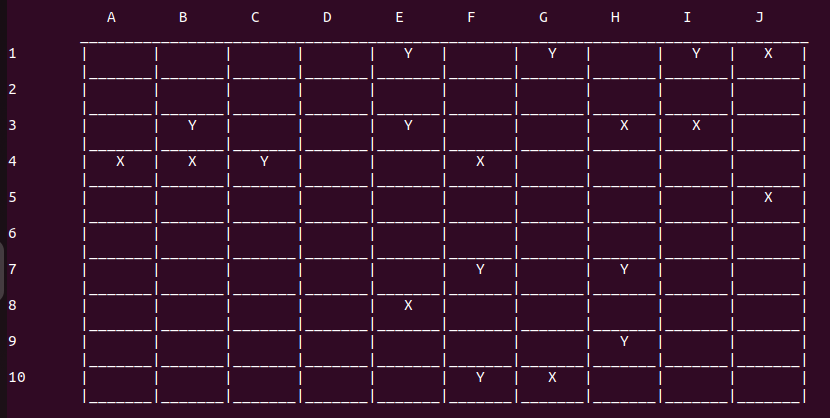
\includegraphics[width=1.0\textwidth,keepaspectratio]{img/Commit9.png}
		%\includesvg{img/automata.svg}
		%\label{img:mot2}
		%\caption{Product backlog.}
	\end{figure}
	\begin{lstlisting}[language=bash,caption={Ejecucion:}][H]
		*********************************

		El soldado con mayor vida del Ejercito 1 es: 
		
		Nombre: Soldado1X1
		Vida: 5
		Fila: 2
		Columna: B
		*********************************
		
		El soldado con mayor vida del Ejercito 2 es: 
		
		Nombre: Soldado2X2
		Vida: 5
		Fila: 9
		Columna: G
		*********************************
		El promedio de puntos de vida del Ejercito 1 es: 
		3.3333333333333335
		*********************************
		El promedio de puntos de vida del Ejercito 2 es: 
		3.0
		*********************************
		El Ejercito 1 ordenando por metodo burbuja: 
		------------------------------------------
		Mostrando Ranking del Ejercito 1 ..... ////// --->
		
		Puesto 1
		Nombre: Soldado1X1
		Vida: 5
		Fila: 2
		Columna: B
		------------------
		
		Puesto 2
		Nombre: Soldado5X1
		Vida: 4
		Fila: 10
		Columna: D
		------------------
		
		Puesto 3
		Nombre: Soldado2X1
		Vida: 3
		Fila: 5
		Columna: G
		------------------
		
		Puesto 4
		Nombre: Soldado0X1
		Vida: 3
		Fila: 5
		Columna: J
		------------------
		
		Puesto 5
		Nombre: Soldado4X1
		Vida: 3
		Fila: 10
		Columna: H
		------------------
		
		Puesto 6
		Nombre: Soldado3X1
		Vida: 2
		Fila: 1
		Columna: C
		------------------
		*********************************
		El Ejercito 2 ordenando por metodo burbuja: 
		------------------------------------------
		Mostrando Ranking del Ejercito 2 ..... ////// --->
		
		Puesto 1
		Nombre: Soldado2X2
		Vida: 5
		Fila: 9
		Columna: G
		------------------
		
		Puesto 2
		Nombre: Soldado5X2
		Vida: 4
		Fila: 10
		Columna: E
		------------------
		
		Puesto 3
		Nombre: Soldado1X2
		Vida: 3
		Fila: 5
		Columna: F
		------------------
		
		Puesto 4
		Nombre: Soldado3X2
		Vida: 3
		Fila: 10
		Columna: A
		------------------
		
		Puesto 5
		Nombre: Soldado4X2
		Vida: 2
		Fila: 4
		Columna: F
		------------------
		
		Puesto 6
		Nombre: Soldado0X2
		Vida: 1
		Fila: 9
		Columna: D
		------------------
		*********************************
		El Ejercito 1 ordenando por metodo insercion: 
		------------------------------------------
		Mostrando Ranking del Ejercito 1 ..... ////// --->
		
		Puesto 1
		Nombre: Soldado1X1
		Vida: 5
		Fila: 2
		Columna: B
		------------------
		
		Puesto 2
		Nombre: Soldado5X1
		Vida: 4
		Fila: 10
		Columna: D
		------------------
		
		Puesto 3
		Nombre: Soldado2X1
		Vida: 3
		Fila: 5
		Columna: G
		------------------
		
		Puesto 4
		Nombre: Soldado0X1
		Vida: 3
		Fila: 5
		Columna: J
		------------------
		
		Puesto 5
		Nombre: Soldado4X1
		Vida: 3
		Fila: 10
		Columna: H
		------------------
		
		Puesto 6
		Nombre: Soldado3X1
		Vida: 2
		Fila: 1
		Columna: C
		------------------
		*********************************
		El Ejercito 2 ordenando por metodo insercion: 
		------------------------------------------
		Mostrando Ranking del Ejercito 2 ..... ////// --->
		
		Puesto 1
		Nombre: Soldado2X2
		Vida: 5
		Fila: 9
		Columna: G
		------------------
		
		Puesto 2
		Nombre: Soldado5X2
		Vida: 4
		Fila: 10
		Columna: E
		------------------
		
		Puesto 3
		Nombre: Soldado1X2
		Vida: 3
		Fila: 5
		Columna: F
		------------------
		
		Puesto 4
		Nombre: Soldado3X2
		Vida: 3
		Fila: 10
		Columna: A
		------------------
		
		Puesto 5
		Nombre: Soldado4X2
		Vida: 2
		Fila: 4
		Columna: F
		------------------
		
		Puesto 6
		Nombre: Soldado0X2
		Vida: 1
		Fila: 9
		Columna: D
		------------------
		*********************************
		El Ejercito 1 es el GANADOR con 3.3333333333333335 puntos
		
	\end{lstlisting}
	\subsection{Estructura de laboratorio 08}
	\begin{itemize}	
		\item El contenido que se entrega en este laboratorio08 es el siguiente:
	\end{itemize}
	\begin{lstlisting}[style=ascii-tree]
	/Lab08	
		"Poner RAMA"

	\end{lstlisting}    
	\section{\textcolor{red}{Rúbricas}}
	
	\subsection{\textcolor{red}{Entregable Informe}}
	\begin{table}[H]
		\caption{Tipo de Informe}
		\setlength{\tabcolsep}{0.5em} % for the horizontal padding
		{\renewcommand{\arraystretch}{1.5}% for the vertical padding
		\begin{tabular}{|p{3cm}|p{12cm}|}
			\hline
			\multicolumn{2}{|c|}{\textbf{\textcolor{red}{Informe}}}  \\
			\hline 
			\textbf{\textcolor{red}{Latex}} & \textcolor{blue}{El informe está en formato PDF desde Latex,  con un formato limpio (buena presentación) y facil de leer.}   \\ 
			\hline 
			
			
		\end{tabular}
	}
	\end{table}
	
	\clearpage
	
	\subsection{\textcolor{red}{Rúbrica para el contenido del Informe y demostración}}
	\begin{itemize}			
		\item El alumno debe marcar o dejar en blanco en celdas de la columna \textbf{Checklist} si cumplio con el ítem correspondiente.
		\item Si un alumno supera la fecha de entrega,  su calificación será sobre la nota mínima aprobada, siempre y cuando cumpla con todos lo items.
		\item El alumno debe autocalificarse en la columna \textbf{Estudiante} de acuerdo a la siguiente tabla:
	
		\begin{table}[ht]
			\caption{Niveles de desempeño}
			\begin{center}
			\begin{tabular}{ccccc}
    			\hline
    			 & \multicolumn{4}{c}{Nivel}\\
    			\cline{1-5}
    			\textbf{Puntos} & Insatisfactorio 25\%& En Proceso 50\% & Satisfactorio 75\% & Sobresaliente 100\%\\
    			\textbf{2.0}&0.5&1.0&1.5&2.0\\
    			\textbf{4.0}&1.0&2.0&3.0&4.0\\
    		\hline
			\end{tabular}
		\end{center}
	\end{table}	
	
	\end{itemize}
	
	\begin{table}[H]
		\caption{Rúbrica para contenido del Informe y demostración}
		\setlength{\tabcolsep}{0.5em} % for the horizontal padding
		{\renewcommand{\arraystretch}{1.5}% for the vertical padding
		%\begin{center}
		\begin{tabular}{|p{2.7cm}|p{7cm}|x{1.3cm}|p{1.2cm}|p{1.5cm}|p{1.1cm}|}
			\hline
    		\multicolumn{2}{|c|}{Contenido y demostración} & Puntos & Checklist & Estudiante & Profesor\\
			\hline
			\textbf{1. GitHub} & Hay enlace URL activo del directorio para el  laboratorio hacia su repositorio GitHub con código fuente terminado y fácil de revisar. &2 &X &2 & \\ 
			\hline
			\textbf{2. Commits} &  Hay capturas de pantalla de los commits más importantes con sus explicaciones detalladas. (El profesor puede preguntar para refrendar calificación). &4 &X &4 & \\ 
			\hline 
			\textbf{3. Código fuente} &  Hay porciones de código fuente importantes con numeración y explicaciones detalladas de sus funciones. &2 &X &2 & \\ 
			\hline 
			\textbf{4. Ejecución} & Se incluyen ejecuciones/pruebas del código fuente  explicadas gradualmente. &2 &X &2 & \\ 
			\hline			
			\textbf{5. Pregunta} & Se responde con completitud a la pregunta formulada en la tarea.  (El profesor puede preguntar para refrendar calificación).  &2 &X &2 & \\ 
			\hline	
			\textbf{6. Fechas} & Las fechas de modificación del código fuente estan dentro de los plazos de fecha de entrega establecidos. &2 &X &2 & \\ 
			\hline 
			\textbf{7. Ortografía} & El documento no muestra errores ortográficos. &2 &X &2 & \\ 
			\hline 
			\textbf{8. Madurez} & El Informe muestra de manera general una evolución de la madurez del código fuente,  explicaciones puntuales pero precisas y un acabado impecable.   (El profesor puede preguntar para refrendar calificación).  &4 &X &2 & \\ 
			\hline
			\multicolumn{2}{|c|}{\textbf{Total}} &20 & &18 & \\ 
			\hline
		\end{tabular}
		%\end{center}
		%\label{tab:multicol}
		}
	\end{table}
	
\clearpage

\section{Referencias}
\begin{itemize}			
	\item \url{https://drive.google.com/file/d/1TbYqdgt7cGTuw_P_ZnkiAXBmPI8YhDMb/view}
\end{itemize}	
	
%\clearpage
%\bibliographystyle{apalike}
%\bibliographystyle{IEEEtranN}
%\bibliography{bibliography}
			
\end{document}